\chapter{JSCsim: A Joint Source--Channel Coding Simulator}
\label{ch:simulator}
\urldef{\jscsimurl}\url{http://ipg.epfl.ch/~kleiner/jscsim/}

For a communication engineer, simulations are an invaluable tool. They can not
only help to verify the correctness of a theoretical result, they can also
 produce results about systems far too complex to be modeled mathematically.

Simulations are often seen as not more than ad-hoc tools. They are
quick-and-dirty programming jobs that have served their purpose once the desired
result has been obtained. According to the rule that the more a program is
likely to change the better it should be structured, however, simulations should
actually be among the most well-structured and thought through pieces of
software. It takes time to plan and write well-structured code, though, but
if the simulation is seen merely as a means to an end, communication engineers
rarely take this time.  As a result, most simulation code will eventually become
so ugly that it is easier to rewrite a new simulation from scratch rather than
to modify the existing one. 

This chapter presents \jscsim, an object-oriented simulator for joint
source-channel coding
schemes.\footnote{\jscsimurl} Its main design goal is to allow rapid testing
of new ideas while simultaneously keeping the code clean and free of
redundancies. 

\jscsim\ is implemented in \matlab\ but could easily be translated to other
languages that support object-oriented programming. Its power lies in its
structure, which relies heavily on the twin paradigms of inheritance and
polymorphism\footnote{\emph{Inheritance} is the capability of a class to
``inherit'' the properties and methods of another class while adding its own
functionality. \emph{Polymorphism} is the capability of a class to appear as and
be used like another class.}. Moreover, this structure can be translated to
communication problems other than joint source-channel coding. 

This chapter is organized as follows. \secref{overview} makes the reader
familiar with \jscsim\ by leading him through a series of hands-on examples and
giving an overview of the implementation.  Thereafter, \secref{reference}
provides a detailed reference and usage manual.  

Before introducing \jscsim, though, the chapter starts with a short example that
illustrates why object oriented programming is so well suited for writing
simulations.

\begin{remark}
  \label{rem:oofundamentals}
  The reader is assumed to be familiar with the fundamentals of object-oriented
  programming (classes, methods, encapsulation, etc.). For those unfamiliar with
  the subject, the Wikipedia article on object-oriented
  programming~\cite{wiki:ooprogramming} provides a good introduction; otherwise
  there are numerous good language-specific introductions around. The examples
  throughout this chapter are in \matlab's programming language; \matlab's
  particular syntax for objects should be easily grasped by someone already
  familiar with object-oriented programming.
\end{remark}

% Install a verbatim shortcut for all the function and variable names that occur
% in the sequel.
\DefineShortVerb{\|}

\section[Object Oriented Programming for Simulations]{Object Oriented
Programming and Simulation: A Great Match}\label{sec:ooforsim}

Imagine that you have written the \matlab\ code in
\lstvref{proceduralsim} to
simulate your freshly devised communication scheme. The function
|run_simulation()| first defines a few relevant parameters and creates a vector
of random source samples. Then, for each SNR value in the defined range, it
calls |encode()| to encode the source symbols into the channel input~|x|, adds
noise, decodes the result~|y|  to produce an estimate~|sh|.  Finally it computes
the empirical MSE and stores it in the vector~|mse|.

\begin{listing}
\begin{Code}
  function mse = run_simulation()
    snr = 10.^(0:.1:5);   % SNR range: 0 to 50 dB
    sv  = 1;              % Source variance
    N   = 100000;         % Sample size
    
    s = get_source_samples(N, sv);
    for k = 1:length(snr)
      x  = encode(s);
      y  = x + gaussian_noise(snr(k));
      sh = decode(y);
      
      mse(k) = mean((s - sh).^2);
    end
  end
\end{Code}
\caption{A hypothetical simulation of a joint source-channel communication
scheme.}
\label{lst:proceduralsim}
\end{listing}

Suppose now that you want to test an alternative decoding method. For example,
you want to see how a maximum likelihood decoder compares to an MMSE decoder. To
this end you implement the alternative decoder in the function |alt_decode()|.
How do you test this function?  You have essentially four possibilities:
\begin{enumerate}
  \item You replace the call to |decode()| in |run_simulation()| by a call to
    |alt_decode()|. The change to the existing code is only minimal. In doing
    so, however, you give up the old version of your code; this is not very
    good since you'll probably want to compare the performance of the new
    decoder to that of the old one and thus keep both versions around.

  \item You copy the contents of |run_simulation()| into a new function called
    |run_alt_simulation()|, replacing the call to |decode()| with a call to
    |alt_decode()|. While
    this approach leaves the old code unchanged and again only requires little 
    programming effort, it results in a lot of duplicate code, which makes your
    program error prone.

  \item You do as in point~2, but then you eliminate duplicate code by putting
    all the common code into separate functions that will be called by both
    |run_simulation()| and |run_alt_simulation()|. This does indeed remove the
    redundancies, but it also requires significant programming effort. Moreover,
    if one day you decide to change the encoder as well, this will probably
    again require a similar amount of effort. 

  \item You add an argument to |run_simulation()| that specifies whether the old
    or the new decoding function should be used, and then you add a test as in
\begin{Code}
  if decode_mode == 0
    sh = decode(y);
  elseif decode_mode == 1
    sh = decode_alt(y);
  end
\end{Code}
    In the example given, |decode()| is called directly from |run_simulation()|,
    so the changes to the code are small (and no redundant code is created).
    However, in a practical simulator the decoding function may be under many
    layers of nested functions, and then all these functions would have to be
    modified to pass on the new parameter. 

    A similar but more sophisticated way would be to set up a way for the
    simulator to read in configuration files and then add a configuration option
    for the decoding method used. This would require a (one-time) programming
    effort but it eliminates the need for options to be passed down from
    function to function. 

    While this fourth method may be better than the first three, it still has
    the drawback that existing simulator code needs to be rewritten.  After
    adding many such options and corresponding conditionals, the code may well
    become difficult to read. Moreover, if someone else is the author of the
    original simulator and he or she releases a new version, all your changes
    will have to be merged into the new version. 
\end{enumerate}

As you can see, none of these options is quite satisfactory. You either lose old
functionality, are left with a lot of duplicate code, or face a significant
restructuring effort.


\subsubsection{The Power of Inheritance}

Suppose now that your programming language supports object-oriented programming
(as \matlab\ does\footnote{at least the more recent releases})
and that you have implemented |run_simulation()|, along with the functions it
calls, as \emph{methods} of the class |Simulation|, as shown in
\lstref{objectsim}. Creating a new simulation with an alternative |decode()|
function now couldn't be easier: just create a \emph{derived class}\footnote{In
many object oriented programming languages, most notably Java, derived classes
are called \emph{subclasses} and base classes are called \emph{superclasses}. As
pointed out by Stroustrup~\cite[\Spg12.2]{Stroustrup1997}, this is somewhat
confusing because the capabilities of a \emph{sub}class form a \emph{super}set
of those of its superclass (and vice versa). Hence in this text we shall stick
to the terms \emph{base class} and \emph{derived class}.} of |Simulation| and
override the |decode()| method, as shown in \lstref{derivedclass}. 

The two versions of the simulation can then be run as follows.
\begin{Code}
  s = Simulation();              % Create class instance
  mse1 = s.run_simulation();     % Call class method
  as = AlternativeSimulation();  % Create class instance
  mse2 = as.run_simulation();    % Call class method
\end{Code}
Because the new class |AlternativeSimulation| inherits everything from
|Simulation| except the overridden method |decode()|, it can be used just like
the original simulation.

\begin{listing}
\begin{Code}
  classdef Simulation
    methods
      function mse = run_simulation()
        ... % as before
      end

      function x = encode(s)
        ...
      end

      function sh = decode(y)
        ...
      end
    end
  end
\end{Code}
  \caption{Object-oriented version of the simulator of \lstref{proceduralsim}.}
  \label{lst:objectsim}
\end{listing}

\begin{listing}
\begin{Code}
  classdef AlternativeSimulation < Simulation
    methods
      function sh = decode(y)
        % Alternative decoder implementation goes here ...
      end
    end 
  end
\end{Code}
  \caption{A new simulation with an alternative decoder is easily implemented by
  deriving a new class from \texttt{Simulation} and overriding the
  \texttt{decode()} method.}
  \label{lst:derivedclass}
\end{listing}

The object-oriented approach has none of the drawbacks of the previous example:
\begin{itemize}
  \item The original simulation remains completely unchanged.
  \item There is no programming effort other than implementing the new method.
  \item There is no redundant code whatsoever.
\end{itemize}

The concept we have exploited here is called \emph{inheritance}, since
|Alternative|\-|Simulation| \emph{inherits} all those methods from
|Simulation| which it doesn't explicitly redefine.  The power of
inheritance is that it allows \emph{old code to call new code}: if |as| is an
instance of |Alternative|\-|Simulation| then a call to |as.run_simulation()|
calls the ``old'' method |run_simulation()| (defined in |Simulation|), which in
turn calls the \emph{new} |decode()| method, without the need to make any
changes to |run_simulation()|. 


In \emph{procedural programming}\footnote{Procedural programming is programming
using functions or \emph{procedures}, as opposed to object-oriented
programming.}, on the other hand, it is only possible for \emph{new code to call old code}: a new
function can call an existing one, but the opposite is not possible without
changing the existing function.  Furthermore, if you want two versions of an
existing function to coexist such that one of them calls a new function (which
is what we tried in our introductory example), this either requires code
duplication (which leads to bugs) or significant programming effort. 

To summarize: one can create two simulations that are identical except for a
single function by the simple act of embedding the functions making up the
simulation in a class and creating a derived class that overrides one of these
functions.


\section{A Short Overview of JSCsim}\label{sec:overview}

This section has two subsections. The first one is for those readers who just
want to see how to \emph{use} \jscsim\ and care less about what goes on behind
the scenes. The second subsection, starting on page~\pageref{sec:impoverview},
presents \jscsim\ from the developer's point of view by explaining the
architecture in a top-down fashion. Depending on the reader's interests, he or
she may safely skip one or the other subsection. 

The best way to read this section may be to read both parts in parallel. Start
by going through the first example of the tutorial, then switch to reading about
the implementation, and continue alternating between the two parts.

\subsection{A Step-By-Step Tutorial}\label{sec:tutorial}

To demonstrate how \jscsim\ helps defining communication schemes and simulating
them, this section presents a number of small hands-on examples. 

\subsubsection{Implementing a Communication Scheme}

\exref{gausssingle} of \chapref{fundamentals} showed that uncoded transmission
is optimal to transmit a Gaussian source across a Gaussian channel if the source
and channel bandwidths are matched. To verify this claim experimentally, let us
implement uncoded transmission in \jscsim. 

\begin{listing}
  \CodeInput{simulator/@UncodedScheme/UncodedScheme.m}
  \caption{Implementation of uncoded transmission.}
  \label{lst:uncoded}
\end{listing}

The code for this is shown in \lstvref{uncoded}.  One can make the following
observations.
\begin{enumerate}
  \item The communication scheme is implemented as a \emph{class} called
    |Uncoded|\-|Scheme| (\lineref{1}). It is derived from the class
    |PracticalScheme|. This is the class that all ``practical'' communication
    schemes are derived from, \ie, communication schemes that can be implemented
    in practice as opposed to merely ``theoretical'' schemes. The so called
    theoretical schemes, of which we will see an example shortly, compute a MSE
    from a mathematical formula (such as $\ssq/(1+\snr)^n$) without simulating
    transmission.

  \item The constructor of |UncodedScheme| receives two parameters
    (\lineref{4}). |sv| is the source variance and |s| is the sequence of source
    symbols that are to be transmitted.\footnote{If you wonder why the
    constructor returns something called \Verb+obj+: this is simply how
    \matlab's syntax specifies the constructor; the returned value is the object
    just created.}

    The constructor of the base class |PracticalScheme| has two additional
    arguments. They are, respectively, the number~$k$ of source symbols encoded
    at a time and the number~$n$ of channel inputs produced from every
    $k$~source symbols. The scheme at hand is for $k = n = 1$, which is why the
    last two parameters passed to |PracticalScheme()| are both~$1$
    (\lineref{5}).

  \item Actual computation is only performed in two methods: |encode()| and
    |decode()|\footnote{Again, the reason why the first argument to both
    \Verb+encode()+ and \Verb+decode()+ is \Verb+obj+ has to do with \matlab's
    syntax. All (non-static) methods of a class must have a first argument that
    refers to the object instance. Here we call it \Verb+obj+ by convention, but
    it could in principle be given any other name. An object's properties are
    accessed from within its methods by prefixing them with `\Verb+obj.+' (cf.
    \lstref{uncoded}).  This is similar to the \Verb+this+ pointer in C++ or
    Java, except that the latter doesn't have to be explicitly given as a method
    argument.}. This makes sense, since a communication scheme is completely
    specified by its encoder and decoder.  For the scheme at hand, these methods
    simply compute $X = \sqrt{P/\ssq} S$ and $\Sh = \sqrt{P \ssq} Y / (P +
    \szq)$.
    
\end{enumerate}


\subsubsection{Performance Analysis}\label{sec:perfanalysis}

Having implemented the class |UncodedScheme|, we would now like to plot its
performance. For this, \jscsim\ has a class called |Performance|\-|Processor|,
which is used as follows.
\CodeInput{figures/matlab/ex_uncoded.minc}
The first two lines define two cell arrays%
\footnote{In \matlab, \emph{cell arrays} are special arrays whose elements can
be of arbitrary types (scalars, vectors, matrices, strings, other cell
arrays, etc.). Cell arrays are specified by listing their elements in curly
braces, as in \texttt{\char`\{1, [2,3], 'foo'\char`\}}.}
with a single entry each.
The first contains the class names of the schemes to plot, and
the second contains a list of parameters for each scheme. Here we only have a
single scheme, |UncodedScheme|. It does not have any parameters, so the
corresponding entry in the parameter list is an empty vector. 

The third line creates an instance of the class |Performance|\-|Processor|,
whose |process()| method we invoke in the fourth line, passing the list of
schemes and parameters. \figvref{uncoded} contains the resulting plot.

\begin{figure}
  \begin{center}
    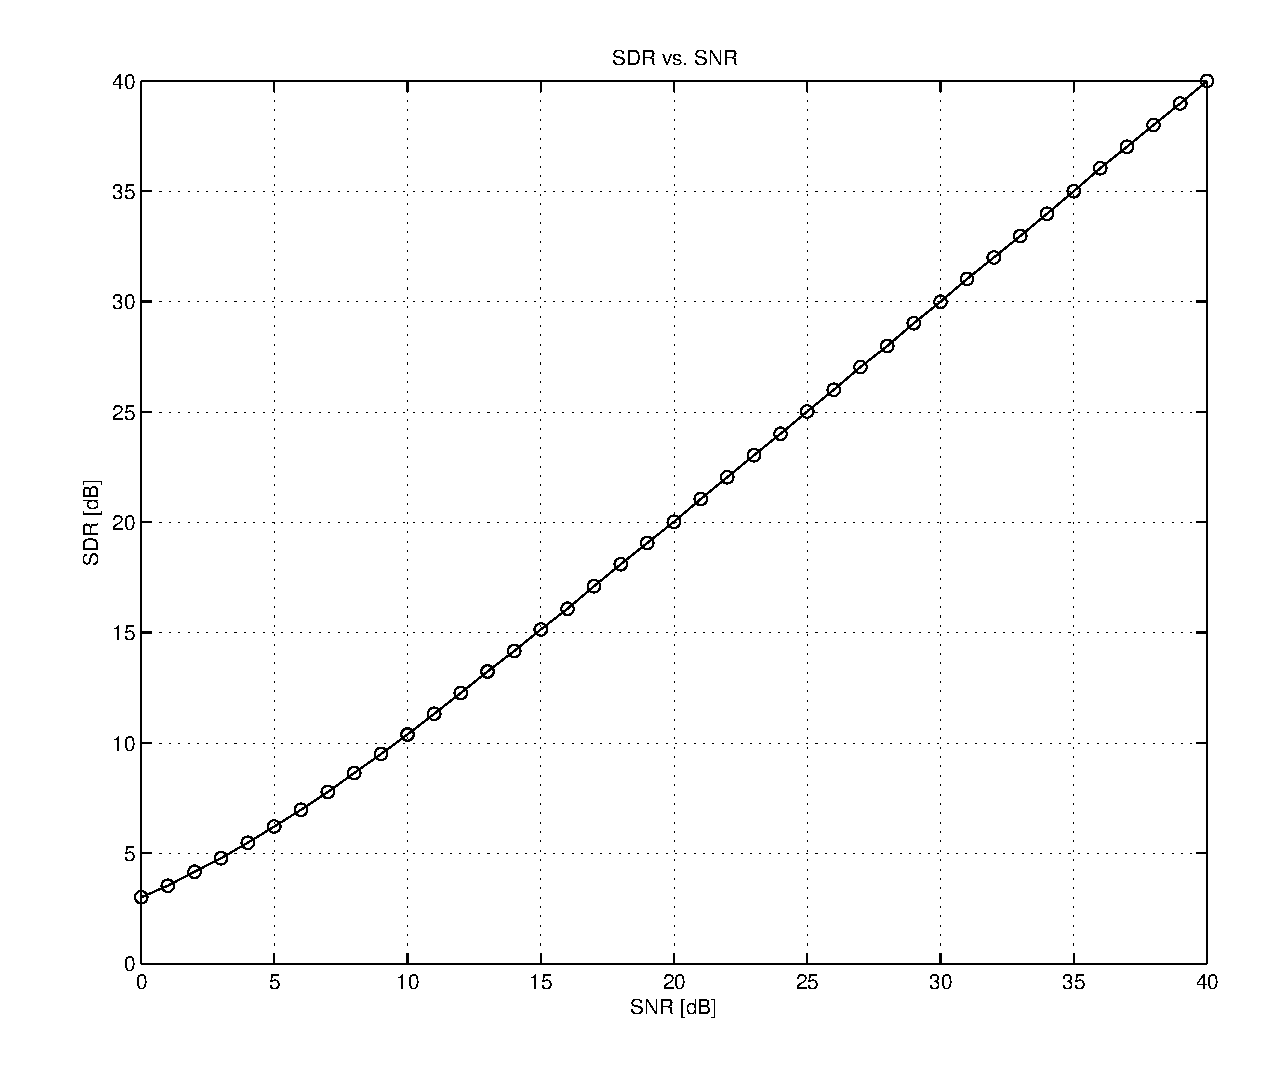
\includegraphics[width=\textwidth]{figures/matlab/ex_uncoded.pdf}
  \end{center}
  \caption{Plot of the SDR resulting from the \texttt{UncodedScheme} class,
  obtained using a \texttt{PerformanceProcessor}.}
  \label{fig:uncoded}
\end{figure}

This was not much work at all. Behind the scenes, however, a lot more was going
on:
\begin{enumerate}
  \item A long sequence of random source symbols was generated.
  \item For a range of SNR values and for each communication scheme, the source
    sequence was encoded using the |encode()| method of our new class,
    Gaussian noise of the appropriate variance was added, and the result was
    decoded using our new |decode()| method.
  \item The average difference between the source sequence and the estimate
    sequence was computed, again for each scheme and for each value of SNR. 
  \item The resulting performance curves were plotted by the
    |Performance|\-|Processor|.
\end{enumerate}
All this work was done by |Performance|\-|Processor| and the base class
|Practical|\-|Scheme|, leaving us free to focus on the essential stuff.
(\secref{impoverview} explains in detail how the above steps are performed.)


\subsubsection{Theoretical Performance}

At this point we have implemented uncoded communication, but we have not
yet verified that it performs indeed optimally. From \chapref{fundamentals} we know
that if there are $n$~channel uses per source symbol then the optimal SDR
is $(1 + \snr)^n$. In \jscsim\ we can implement this as a ``theoretical''
communication scheme: this is a communication scheme that doesn't actually do
any encoding or decoding, but simply computes a theoretical MSE for a 
given SNR.

\begin{listing}
\begin{Code}
  classdef ShannonScheme < TheoreticalScheme
    properties
      n         % The number of channel uses per source symbol.
    end

    methods (Access = 'public')
      function obj = ShannonScheme(sv, s, n)
        
        % Call base class constructor.
        obj = obj@TheoreticalScheme(sv, s);

        % Set class-specific parameters.
        obj.n = n;
      end
    end

    methods (Access = 'protected')
      % This function is called whenever the SNR is changed and so
      % the MSE needs to be recomputed.
      function update_mse(obj)
          obj.mse = obj.sv / (1 + obj.snr)^obj.n;
      end
    end
  end
\end{Code}
  \caption{A ``theoretical'' communication scheme does not perform any
  actual encoding or decoding, but rather computes the theoretically optimal MSE
  for a given SNR.}
  \label{lst:shannonscheme}
\end{listing}

The resulting \matlab\ code is given in \lstvref{shannonscheme}. We can make the
following observations.
\begin{enumerate}
  \item The class |ShannonScheme| is derived from |TheoreticalScheme| rather
    than from |PracticalScheme| as in the previous example (\lineref{1}). This
    is because unlike practical schemes, theoretical schemes do not have
    |encode()| or |decode()| methods. 
    
  \item |ShannonScheme| has a single parameter~|n|, the number of channel uses
    per source symbol, which it receives as an argument of its constructor
    (\lineref{7}).

  \item The method |update_mse(obj)| (\lineref{20}) is the heart of this
    class. This method is called by the base class whenever the SNR is
    changed. Here it computes $\ssq / (1
    + \snr)^n$, which is the theoretically optimal MSE for the given SNR
    (cf.~\chapref{fundamentals}).
    
  \item |update_mse()| accesses the |snr| property (\lineref{21}), even though
    we never defined this property. This is because the property is set by the
    base class, so that all derived classes have access to the SNR.
\end{enumerate}

To plot the performance of both |UncodedScheme| and |ShannonScheme| on the same
plot, we can use the |Performance|\-|Processor| as before:
\CodeInput{figures/matlab/ex_shannonscheme.minc}
The only difference to the previous example is that the |schemes| array now has
two elements and that we need to specify the parameter $n=1$ for
|ShannonScheme|.  This parameter will be passed to the constructor of
|ShannonScheme| as its third argument.

The resulting plot is shown on \figvref{shannonscheme} and confirms that uncoded
transmission is indeed optimal. Note that a legend has automatically been added
because we are plotting the performance of more than one communication scheme.

\begin{figure}
  \begin{center}
    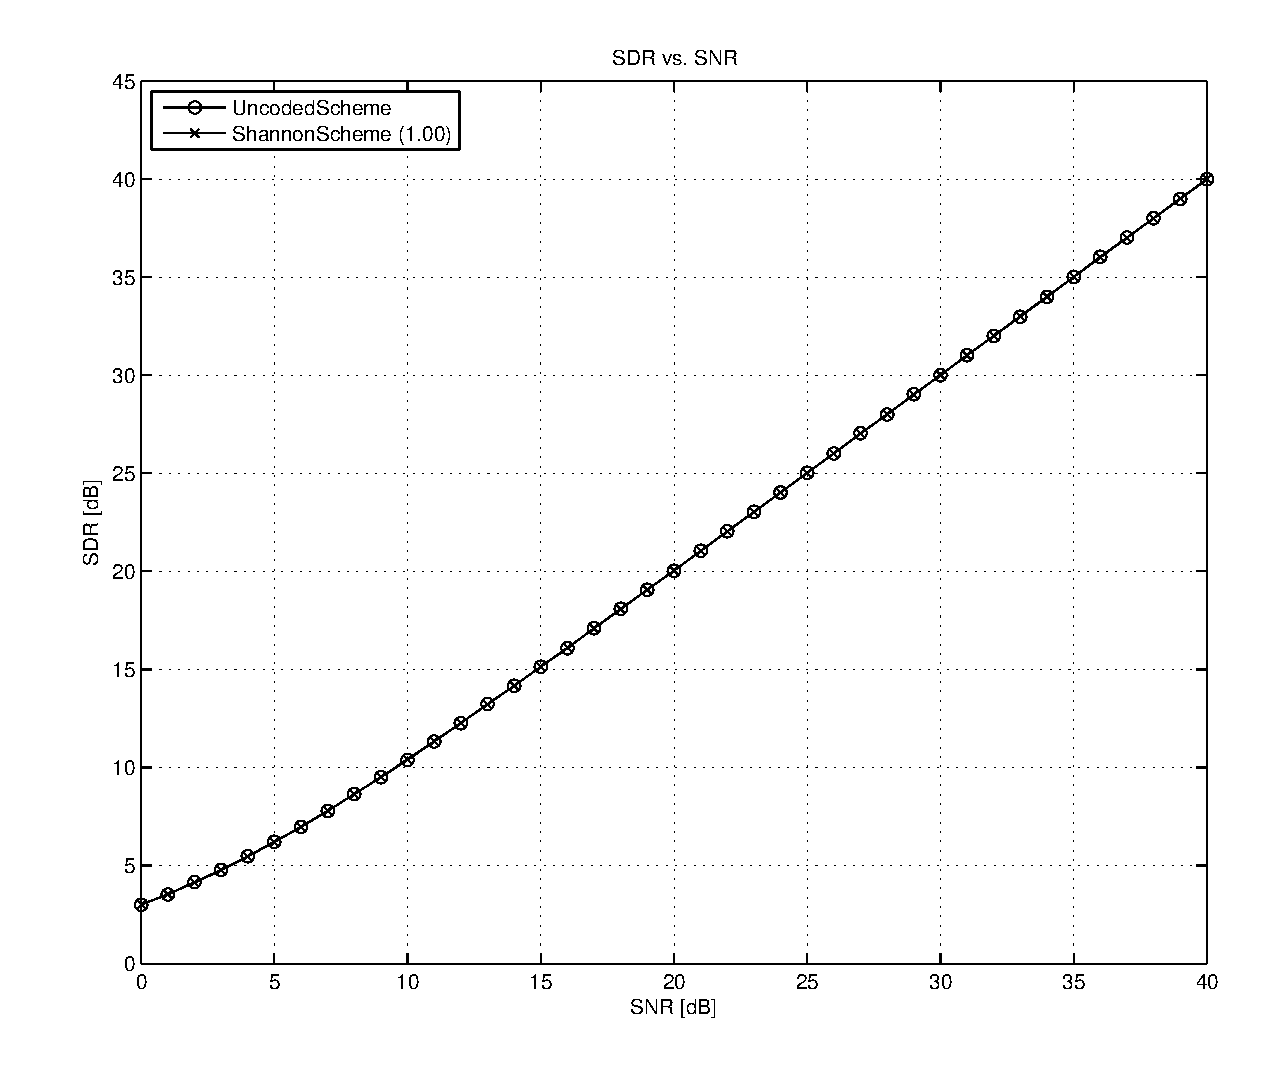
\includegraphics[width=\textwidth]{figures/matlab/ex_shannonscheme.pdf}
  \end{center}
  \caption{Comparing the theoretically optimal performance and the performance
  of uncoded transmission. The two curves coincide, experimentally confirming
  that uncoded transmission is optimal for the transmission of a Gaussian source
  across a Gaussian channel.}
  \label{fig:shannonscheme}
\end{figure}


\subsubsection{Alternative Output Formats}

In the examples we saw so far, the performance processor just launched a
standard \matlab\ figure window with the performance plot. Often, though, you
may not only want to look at the plot on the screen but also use it in a report
or in a paper. For this, \jscsim\ has the concept of \emph{output modules}. An
output module is a class that implements a rudimentary set of plot capabilities.

The default output module is called |MatlabPlotModule| and uses \matlab's plot
command to display a figure window. Alternatively, to save the performance plot
in a PDF file, for instance, the default output module can be replaced by a
|MatlabFilePlotModule|. Instead of displaying the plot in a window, this output
module saves it in a file.  Continuing our previous example, we can use it as
follows.
\begin{Code}
  ...  % Define list of schemes and parameters.
  pp = PerformanceProcessor();
  pp.output_module = MatlabFilePlotModule();
  pp.output_module.fn = 'myplot.pdf';
  pp.process(schemes, parameters);  % Saved to myplot.pdf.
\end{Code}
In \lineref{3} a new output module of type |MatlabFilePlotModule| is
created and attached to the performance processor. Since this output module
writes its output to a file, we have to specify a file name in \lineref{4}.
Afterwards, we can call |process()| just as before.\footnote{Unsurprisingly,
Figures~\ref{fig:uncoded} and~\ref{fig:shannonscheme} have in fact been created
using \Verb+Matlab+\-\Verb+FilePlotModule+.}

\urldef{\pgfplotsurl}\url{http://pgfplots.sourceforge.net/}
There is another output module, called |PGFPlotsOutputModule|. It produces a
file containing \LaTeX\ code to be used with the \pgfplots\
package\footnote{\pgfplotsurl}. To use it, just replace |MatlabFilePlotModule|
in the above example by |PGFPlotsOutputModule| and set \eg
\begin{Code}
  pp.output_module.fn = 'myplot.tex';
\end{Code}
The resulting file can then be included in a \LaTeX\ file, provided that the
|pgfplots| package has been loaded.  The result is shown on \figref{uncodedpgf}.
Admittedly, plots created by \pgfplots\ fit in nicer with the \LaTeX\
layout, and their labels are more readable than those of
Figures~\ref{fig:uncoded} and~\ref{fig:shannonscheme}.

\begin{figure}
  \begin{center}
    \input{figures/matlab/ex_uncodedpgf.tex_t}
  \end{center}
  \caption{Using the \texttt{PGFPlotsOutputModule}, one can save the simulation
  output as \TeX\ commands for the \pgfplots\ package, which can then be
  included in a \LaTeX\ source file.}
  \label{fig:uncodedpgf}
\end{figure}


\subsubsection{Analysis Using Scheme Processors}

The performance processor we have used to plot the performance in the previous
examples is a particular type of \emph{scheme processor}. The idea behind scheme
processors is to separate the implementation and the simulation of communication
schemes.

A scheme processor takes a list of schemes along with the corresponding
parameters, simulates these for a range of SNR values, and gathers data from
each simulation run. 

Each scheme processor is derived from the class |SchemeProcessor|. It must
implement three methods:
\begin{itemize}
  \item |initialize()| to allocate space for the data gathered;
  \item |save_scheme_data()| to collect data after each simulation run; and
  \item |post_process()| to post-process the gathered data, which usually just
    means to plot it.
\end{itemize}
This is illustrated by the simplified implementation of |PerformanceProcessor|
in \lstvref{perfproc}. This class has a single property, |mse| (\lineref{4}),
where it stores the mean squared errors gathered in each simulation run. In its
|initialize()| method, |mse| is initialized to a big all-zero matrix of the
right size. In the method |save_scheme_data()|, the communication scheme just
simulated (passed as the argument |scheme|) is queried by calling its
|compute_mse()| method (\lineref{13}) and the result is stored in the matrix
|mse|. Finally, |post_process()| plots the MSE of all processed schemes.

\begin{listing}
  \CodeInput{figures/matlab/PerformanceProcessor_ex.minc}
  \caption{Simplified implementation of the \texttt{PerformanceProcessor}
  class.}
  \label{lst:perfproc}
\end{listing}

For another example of a performance processor, consider the hybrid
communication scheme implemented as |Hybrid2DScheme| in \lstref{hybridscheme}.
In this communication scheme, each source symbol~$S$ is split into a discrete
part~$Q$ and a continuous part~$E$ (lines~10--11), which are then transmitted
across two
channel uses (lines~13--14).  The decoder computes the source estimate~$\Sh$
from the separate estimates~$\Qh$ and~$\Eh$ (lines 18--20). (This is similar to
the communication schemes introduced in \chapref{mindelbwex}.)

\begin{listing}
\begin{Code}
  classdef Hybrid2DScheme < PracticalScheme
      
      properties (Access = 'protected')
          q
          qh
      end
      
      methods (Access = 'protected')
          function x = encode(obj, s)
              obj.q = discrete_part(s);
              e = continuous_part(s);
              
              x(1, :) = scale_to_power_constraint(obj.q);
              x(2, :) = scale_to_power_constraint(e);
          end
          
          function sh = decode(obj, y)
              obj.qh = estimate_qh(y);
              eh = estimate_eh(y);
              sh = combine_estimates(obj.qh, eh);
          end

          % Other methods here ...
      end

      % Methods for scheme processors to access simulation data.
      methods (Access = 'public')
          function q = compute_q(obj)
              q = obj.q;
          end
          
          function qh = compute_qh(obj)
              qh = obj.qh;
          end
      end
  end
\end{Code}
\caption{Simplified implementation of a hybrid communication scheme. Note how
\texttt{qh} and \texttt{eh} are saved as class properties, so that they can be
accessed by a scheme processor through the respective \texttt{compute\_*}
methods.}
\label{lst:hybridscheme}
\end{listing}

A question of interest is the behavior of the average error $\E[(Q - \Qh)^2]$ as
a function of the SNR. The scheme processor |Hybrid2DProcessor| in
\lstref{hybridprocessor} solves this task in a few small steps. It is very
similar to the |PerformanceProcessor| of \lstref{perfproc}, except that
different variables are accessed in \lineref{13}. Since the corresponding
communication scheme class, |Hybrid2DScheme|, saves |q| and~|qh| as class
properties and implements public |compute_*| methods for these properties,
the |save_scheme_data()| method of the new scheme processor can easily access
these and compute the corresponding error.

\begin{listing}
\begin{Code}
  classdef Hybrid2DProcessor < SchemeProcessor
      
      properties (Access = 'protected')
          qe
      end
      
      methods (Access = 'protected')
          function initialize(obj)
              obj.qe = zeros(obj.nb_schemes(), length(obj.snr));
          end
          
          function save_scheme_data(obj, scheme, j, k)
              obj.qe(j, k) = mean((scheme.compute_q() - ...
                scheme.compute_qh()).^2);
          end
          
          function post_process(obj)
              % Plot qe vs. SNR ...
          end
      end
  end
\end{Code}
\caption{A scheme processor to plot the estimation error of the discrete part in
a hybrid communication scheme.}
\label{lst:hybridprocessor}
\end{listing}


\subsection{Implementation Overview}\label{sec:impoverview}

\subsubsection{Design Philosophy}

The design philosophy behind \jscsim\ is to separate the implementation of a
communication strategy and the simulation thereof. The end user should be able
to concentrate either on implementing the communication scheme or writing the
code that processes it during simulation, but shouldn't have to think about both
tasks at the same time.  For this reason, the core classes that make up \jscsim\
are divided into two categories. In the first category are the \emph{scheme
classes} (or simply 'schemes'), which are classes that implement communication
schemes and have the class |Scheme| as their common ancestor. \secref{ooforsim}
already covered why it makes sense to implement communication schemes as
classes. 

The second category consists of  \emph{scheme processors}, which are classes
that implement the processing of a particular quantity (such as the MSE) during
the simulation of a single or of a family of communication schemes. Scheme
processors derive from the common ancestor class |SchemeProcessor|. What is the
motivation behind organizing the processing code in this way? The ``processing''
of a communication scheme consists of two steps:
\begin{enumerate}
  \item simulating the scheme by feeding the encoder with randomly generated
    source samples, transforming the encoder output by simulating a noisy
    channel (\eg, by adding Gaussian noise), and passing the channel output to
    the decoder
  \item gathering relevant data, \eg, the mean squared error or other
    performance criteria, after the simulation has run, and displaying it
\end{enumerate}
The base class |SchemeProcessor| essentially implements the first
step. The second step is implemented in derived classes such as
|Performance|\-|Processor| (which computes and plots the achieved SDR). This
structure makes it possible to quickly implement new processor classes to
analyze arbitrary quantities of a communication scheme or of a set of schemes,
as the examples in the previous section show.

Based on the reasonable assumption that you implement a particular
communication scheme in \jscsim\ because you eventually want to simulate it, you never directly instantiate a scheme class. Rather, you create a
particular scheme processor (by instantiating a class derived -- directly or
indirectly -- from |SchemeProcessor|) and call its |process()| method. Note that
you cannot create an instance of the base class |SchemeProcessor| since the
latter contains abstract methods\footnote{An \emph{abstract method} is a
method that is declared in a class but not implemented. For example, a class
\texttt{Shape} might declare an abstract method \texttt{compute\_area()}, which
must be implemented by the derived classes \texttt{Circle}, \texttt{Square}, and
\texttt{Triangle}. A class that has abstract methods cannot be instantiated.}
and serves only as a template for scheme processors. The
example on page~\pageref{sec:perfanalysis} shows how a performance processor,
which is a particular type of scheme processor, is used to plot the
SDR achieved by a communication scheme.

The interaction between scheme processors and scheme classes is illustrated in
\figvref{schemeprocinteraction}.  When you first create an instance of a scheme
processor, it generates and saves a random source sequence of a default
variance.\footnote{By default, the source samples are normally distributed, but
this behavior may easily be changed by a derived class.} Next you call the
|process()| method of the scheme processor, passing a list of schemes (\ie,
names of scheme classes) and a list of parameters for each scheme (cf.~the
example on page~\pageref{sec:perfanalysis}). (A scheme can have any number of
parameters, like for instance the number of channel input symbols produced per
source symbol.) Internally, the scheme processor then creates an instance of
each specified scheme, passing the source sample sequence to each one's
constructor. Because all schemes operate on the same source sequence, a fair
comparison is guaranteed. 

\begin{figure}
  \begin{center}
    \input{figures/schemeprocessor.tex_t}
  \end{center}
  \caption{Interaction between a scheme processor and scheme classes. For each
  scheme, the scheme processor repeatedly calls the scheme's \texttt{set\_snr()}
  method with different SNR values and then gathers the resulting simulation
  data.}
  \label{fig:schemeprocinteraction}
\end{figure}

A scheme processor has a list of SNR values for which each scheme is to be
processed. By default, it runs from 0dB to 40dB with increments of~1dB. For
each SNR value and for each scheme, the scheme processor calls the scheme's
|set_snr()| method, passing the SNR value as an argument (cf.~\lineref{13} in
\lstvref{schemeclass}). 

When a scheme's |set_snr()| method is called, it stores the new SNR in its |snr|
property and calls the |snr_updated()| method. The job of this method is to
update the state of the scheme object to reflect the new SNR. For example, after
a call to a scheme object's |set_snr()| method, its |mse| property should be set
to the mean square error that the scheme achieves with the given SNR. How
exactly a scheme updates its state when |snr_updated()| is called is up to the
implementation. As we will see below, though, the procedure is very similar for
a large class of schemes, of which \jscsim\ takes advantage. 

After calling a scheme's |set_snr()| method, a scheme processor can access
the scheme's |mse| property (for instance) via the scheme's |compute_mse()|
method (which we will see shortly). A scheme processor whose purpose it is to
track the MSE achieved by a particular scheme thus alternatingly calls
|set_snr()| and |compute_mse()| and stores the MSE for each SNR. This is
precisely what the class |PerformanceProcessor| does. 

Other scheme processors collect different data. For instance, the
|Hybrid2DProcessor| in \lstvref{hybridprocessor} separately computes and stores
the errors from the discrete and the continuous transmission rounds for the
hybrid scheme in \lstref{hybridscheme}.

The remainder of this section looks in detail at the implementation of the
scheme classes and of the performance processors.


\subsubsection{Scheme Classes}

The common ancestor of all scheme classes is called |Scheme| and is shown in
\lstvref{schemeclass}. It defines the most rudimentary features that all
communication scheme implementations must have. 

\begin{listing}
\CodeInput{figures/matlab/Scheme.minc}
\caption{The \texttt{Scheme} class is the base class from which all
communication scheme classes are derived.}
\label{lst:schemeclass}
\end{listing}

The class definition starts in \lineref{1}. It is a \matlab\ convention that any
class whose internal state can change over time (as is the case for all classes
considered here) must be derived from the |handle| class, but this is only a
technical detail and of no importance in the sequel.

As we will shortly see in detail, \jscsim\ divides communication schemes into
two types: theoretical schemes and practical schemes. Schemes of both
types are (indirectly) derived from |Scheme|, so |Scheme| defines only the
behavior common to both types, which consists essentially of the methods to set
the SNR and to retrieve the MSE. 

Every communication scheme has access to the three properties defined in
lines~2 to~6: the source variance, the SNR, and the incurred mean squared error.
The source variance is passed via the constructor whenever a class derived from
|Scheme| is instantiated (\lineref{9}). The SNR is set by |set_snr()|
(\lineref{13}). The MSE property is not set by any of the class' methods; it
will be the job of the derived classes to update this property in their
|snr_updated()| method. 

You may wonder why the constructor in \lineref{9} receives an argument~|s| but
ignores it. The reason is that a scheme processor always passes the list of
source symbols to a scheme it processes, even if it is a theoretical scheme that
does not use the source symbols. More about this is explained further below.

We have already mentioned the method |set_snr()| (\lineref{13}). It is called by
a scheme processor whenever the communication scheme is to be simulated for a
new SNR. This method first saves the new SNR in its |snr| property
(\lineref{14}) and then calls the abstract method |snr_updated()| to inform
derived classes about the changed SNR.

The method |compute_mse()| allows scheme processors to access a scheme's
|mse| property. (Because the property is declared as \emph{protected} (cf.
\lineref{2}), it cannot be directly accessed from outside the class, only
through a method.) 

Line~24 declares the abstract method |snr_updated()|. Because |Scheme| itself
does not implement this method, the class cannot be instantiated directly.
Instead, any class derived from |Scheme| must implement
|snr_updated()|.\footnote{It is not quite true to say that any class derived
from \texttt{Scheme} \emph{must} implement the abstract method
\texttt{snr\_updated()}. A derived class is free not to implement the method; if
it does not implement it, however, it remains itself an abstract class and
cannot be instantiated either. A class can only be instantiated if it implements
all abstract methods defined by any of its ancestors. Of course, if a class
\texttt{X} has already implemented an abstract class declared in one of its
ancestors, then classes derived from~\texttt{X} no longer need to
implement the abstract method themselves because they inherit the implementation
from~\texttt{X}.}


\subsubsection{Theoretical Schemes}

Theoretical schemes could also be called ``virtual'' schemes. They are not
actual communication strategies, they rather compute theoretical values for a
given SNR. The purpose of a theoretical scheme is to compare the behavior of a
communication scheme to a theoretically expected behavior. For an example, see
the class |ShannonScheme| in \lstvref{shannonscheme}.

The implementation of |TheoreticalScheme| is given in
\lstvref{theoreticalscheme}. The class directly derives from |Scheme|
(\lineref{1}); its constructor does nothing except call the base class
constructor, passing on the arguments (\lineref{4}). 

\begin{listing}
  \CodeInput{figures/matlab/TheoreticalScheme.minc}
  \caption{Simplified implementation of the class \texttt{TheoreticalScheme}.}
  \label{lst:theoreticalscheme}
\end{listing}

As mentioned before, classes derived from |Scheme| must implement the method
|snr_updated()|. The implementation in |TheoreticalScheme| is quite simple:
|snr_updated()| just calls |update_mse()|. The latter is itself an abstract
method of |TheoreticalScheme|. This way of structuring the class is just a
programmatical way of saying ``the only thing a theoretical scheme needs to do
when a new SNR is set is to compute the MSE as a function of the SNR''.
Listing~\ref{lst:shannonscheme} provides a sample implementation of
|compute_mse()|. 


\subsubsection{Practical Schemes}

As opposed to theoretical schemes, practical schemes are classes that actually
\emph{implement} a communication scheme. When the SNR is updated, a practical
scheme must simulate encoding, transmission, and decoding of the source symbols.
Since this procedure (except the particularities of encoding and decoding) is
the same for all practical schemes, it is implemented in the class
|PracticalScheme|, from which implementations of particular communication
schemes can then be derived. The actual encoding and decoding functions are
declared abstract in |PracticalScheme|, \ie, classes that implement
communication strategies need only implement these two methods. 

A simplified version of |PracticalScheme| is shown in \lstvref{practicalscheme}.
Its |snr_updated()| method performs exactly the steps mentioned above: the
source sequence~|s| is encoded into a channel input sequence~|x| (\lineref{5}),
transmission is simulated by adding Gaussian noise to~|x| (\lineref{8}), and
the channel output~|y| is decoded to yield the estimate sequence~|sh|
(\lineref{11}).  Finally, the MSE is computed and stored in the |mse|~property
(\lineref{14}).  This is the precisely the property that a performance processor
accesses when it calls the scheme's |compute_mse()| method (which we saw in the
base class |Scheme|). 

\begin{listing}
  \CodeInput{figures/matlab/PracticalScheme.minc}
  \caption{A simplified implementation of \texttt{PracticalScheme}. The methods
  \texttt{encode()} and \texttt{decode()} are declared abstract and must be
  implemented by derived classes.}
  \label{lst:practicalscheme}
\end{listing}

The methods |encode()| and |decode()| are the defining feature of a
communication scheme. There is no ``default'' encoder and decoder, hence
|PracticalScheme| does not provide an implementation of them but declares them
as abstract. They must be implemented by derived classes (such as
|UncodedScheme| in \lstvref{uncoded}).


\subsubsection{Scheme Processors}

Scheme processors instantiate a list of scheme classes and process them for a
range of SNR values. All scheme processors derive from |SchemeProcessor|, a
simplified implementation of which is given in \lstvref{schemeprocessor}. 

\begin{listing}
  \CodeInput{figures/matlab/SchemeProcessor.minc}
  \caption{Simplified implementation of the \texttt{SchemeProcessor} class.}
  \label{lst:schemeprocessor}
\end{listing}

All scheme processors have at the three properties defined in lines~3--5. The
vector~|s| stores the source sequence, which is created in the constructor upon
instantiation (\lineref{16}). The other two properties, |schemes| and
|parameters|, hold the list of schemes to process and the corresponding
parameters, respectively. 

|SchemeProcessor| also has three \emph{public} properties. Because they are
declared \emph{public}, they can be changed from outside the class; they allow
the user of a scheme processor to control the latter's behavior. The meaning of
these three properties should be self-evident from the code; for details see
\secref{reference}.

A scheme processor is launched by calling its |process()| method. This method
has two arguments, |schemes| and |parameters|. Both are cell arrays that
specify the schemes to be processed (\ie, the names of the respective classes)
and the parameters for each scheme, respectively. See
page~\pageref{sec:perfanalysis} for an example of how to call |process()|.

|process()| first saves the schemes and parameters in the respective class
properties (\lineref{20} resp.~lines~4--5). Then it calls the |initialize()|
method (\lineref{21}). This abstract method allows scheme processor
implementations to do things before the actual processing starts. The most
common use of this function is to allocate a data structure that will hold the
data gathered from the schemes (for an example, see the implementation of
|PerformanceProcessor| in \lstvref{perfproc}).  The |do_processing()| method
(line~22 resp.~28) then performs the actual processing of the schemes, we will
look at it in detail shortly. Finally, the abstract method |post_process()| is
called (\lineref{23}). In this method, derived classes can for example display
the data gathered from the schemes, or save it in a file, etc.

The function |do_processing()|, which starts in \lineref{28}, is the core of
|SchemeProcessor|. In two nested \emph{for} loops it traverses the list of
schemes and the range of SNR values. For each scheme and for each SNR it first
calls |set_snr()| (we have already seen above what this method does), and then
it calls the abstract method |save_scheme_data()| (\lineref{35}). In their
implementation of this key method, derived classes determine which data to save
about the scheme. For example, the performance processor on
page~\pageref{sec:perfanalysis} uses it to store the MSE. (The arguments of
|save_scheme_data()| are described in detail in \secref{reference}.)


\subsubsection{Summary}

The preceding paragraphs have hopefully given the reader a good overview of how
\jscsim\ is implemented. Naturally, some details have been swept under the rug.
For instance, |PracticalScheme| also helps in arranging the source sequence in
blocks of $k$~source symbols if a scheme encodes more than one source symbol at
once, and scheme processors use a slightly more involved method to store schemes
and their parameters internally than the one shown. For these details, the
reader so inclined is invited to peruse the source code, available at
\jscsimurl.


\section{Reference}\label{sec:reference}

This reference section explains in detail how to use \jscsim\ to implement new
communication schemes, how to simulate them, and how to build custom scheme
processors. 


\subsection{Communication Schemes}

There are two kinds of communication schemes in \jscsim: \emph{theoretical}
schemes and \emph{practical} schemes. Theoretical schemes compute the MSE for a
given SNR by computing some function of it without simulating anything. They
allow you to compare the performance of a particular communication scheme with a
theoretical value, as for example the |ShannonScheme| in \lstref{shannonscheme}.
On the other hand, practical schemes (like the one in \lstref{uncoded})
determine the MSE by actually simulating communication.


\subsubsection{Theoretical Schemes}

Theoretical communication schemes are implemented as classes derived from
|TheoreticalScheme|. Any class derived from |TheoreticalScheme| must implement
the following methods.

\begin{method}{\meta{class name}(\oarg{sv}, \oarg{s}
  [, \opt{\meta{parameters}}]) (public)}
  This is the constructor of the class. The first two arguments are the source
  variance +sv+ and the source sample sequence~+sv+, which must be passed on to
  the base class constructor, \ie, by calling
  \begin{Code}
  obj@TheoreticalScheme(sv, s);
  \end{Code}

  If a theoretical scheme has parameters, such as the bandwidth expansion
  factor~|n| of |ShannonScheme| (cf.~\lstref{shannonscheme}), they must be
  specified as additional arguments to the constructor.
\end{method}

\begin{method}{update_mse(\obj) (protected)}
    This method is called by the base class whenever the SNR is changed. It
    must update the |mse| property based on the value of the |snr| property.
    For example, the |update_mse()| method of |ShannonScheme| sets |mse| to be
    $\ssq / (1 \normalplus \snr)^n$.
\end{method}


\subsubsection{Practical Schemes}

Practical communication schemes are implemented as classes derived from
|PracticalScheme|. Any class derived from |PracticalScheme| must implement the
following methods.
\begin{method}{\meta{class name}(\oarg{sv}, \oarg{s}
  [, \opt{\meta{parameters}}]) (public)}
  This is the constructor of the class. The first two arguments are the source
  variance +sv+ and the source sample sequence +s+, which must be passed on to
  the base class constructor. The base class constructor has two more arguments,
  which are the number $k$~of source symbols encoded at a time, and the number
  $n$~of channel symbols produced for every $k$~source symbols.
  Depending on the scheme, these can be fixed values (as in |UncodedScheme| in
  \lstref{uncoded}) or variable parameters of the scheme itself.

  \codeexample A scheme that only works for $1$:$2$ bandwidth expansion would
  have a constructor similar to the following.
  \begin{Code}
  function obj = MyScheme1(sv, s)
    obj@PracticalScheme(sv, s, 1, 2);
    % rest of constructor ...
  end
  \end{Code}
  On the other hand, a scheme that encodes one source symbol into $n$~channel
  inputs, where $n$~is arbitrary, would define a constructor like this.
  \begin{Code}
  function obj = MyScheme2(sv, s, n)
    obj@PracticalScheme(sv, s, 1, n);
    % rest of constructor ...
  end
  \end{Code}
\end{method}

\begin{method}{\oarg{x} = encode(\obj, \oarg{s}) (protected)}
  This method receives +s+, a matrix of source samples with $k$~rows, and must
  return a matrix~+x+ with $n$~rows and the same number of columns as~+s+.
\end{method}

\begin{method}{\oarg{sh} = decode(\obj, \oarg{y}) (protected)}
  This method receives the channel output~+y+ as a matrix with $n$~rows and
  must return a matrix~+sh+ with $k$~rows of source estimates
\end{method}

In addition, derived classes may want to override
|update_variable_parameters()|.
\begin{method}{update_variable_parameters(\obj) (protected)}
  In this method, which is called whenever the SNR changes, derived classes can
  update any of their own properties that depend on the SNR. It
  is important that if a derived class overrides this method, it must first
  call the base class method, \ie,
  \begin{Code}
  function update_variable_parameters_(obj)
    % Call base class version.
    update_variable_parameters@PracticalScheme(obj); 
    % Your code here ...
  end
  \end{Code}
\end{method}

To allow a scheme processor to track a particular property of a communication
scheme, the property must be made accessible. This is normally done by  writing
a |compute_*| method. We have already seen the example of the |compute_mse()|
function, which is defined by the class |Scheme|. The class |PracticalScheme| in
addition implements the following such methods.

\begin{method}{x = compute_x(\obj) (public)}
  Returns the channel input sequence.
\end{method}

\begin{method}{y = compute_y(\obj) (public)}
  Returns the channel output sequence.
\end{method}

\begin{method}{sh = compute_sh(\obj) (public)}
  Returns the sequence of source estimates.
\end{method}

Any derived class must thus implement a |compute_*| function for each
property it wants to make accessible to a scheme processor.


\subsection{Scheme Processors}

Scheme classes are usually not handled directly; rather, they are processed by
a \emph{scheme processor}. Scheme processors evaluate a set of communication
schemes for a range of SNR values and store and process the data gathered during
the simulations.

All scheme processors are implemented as classes derived from |SchemeProcessor|.
To process a communication scheme (or a set of schemes) you never directly use a
|SchemeProcessor| object. Instead, you either use an existing derived class such
as |PerformanceProcessor|, or you implement a custom scheme processor. 


\subsubsection{General Aspects}

The behavior of all scheme processors can be controlled through the following
properties, defined in the class |SchemeProcessor|.
\begin{property}{snr (public; default ?10.^(0:.1:4)?)}
  A vector that specifies the SNR range over which the
  communication schemes are simulated. By default it is set to the range
  0dB to 40dB with increments of 1dB. 
\end{property}

\begin{property}{N (public; default ?100000?)}
  The length of the random source sample sequence.
\end{property}
  
\begin{property}{verbose (public; default ?false?)}
  If this parameter is set to true, various status and debugging messages are
  displayed during the simulations.
\end{property}

\begin{property}{output_module (public)}
  This is the output module used by the scheme processor to display its
  results (see the section on output modules). The default output module is
  |MatlabPlotModule|.
\end{property}

\begin{property}{legendmode (public, default \texttt{'auto'})}
  This property determines the behavior of the |plot_vs_csnr()| and
  |plot_|\-|vs_|\-|csnr_|\-|db()| functions (cf.~the definition of |post_process()| below).
  If |legendmode| is set to |'on'|, a legend is always displayed. If it is set
  to |'off'|, a legend is never displayed. If it is set to |'auto'|, a legend is
  only displayed if more than one scheme is plotted.
\end{property}

All scheme processors are launched using the |process()| method.
\begin{method}{process(\obj, \oarg{schemes}, \oarg{parameters}) (public)}
  Process the specified schemes for the specified parameters. The cell array
  +schemes+ lists the schemes to be processed; each of its elements is a string
  equal to the name of a scheme class.

  The cell array +parameters+ has the same number of elements as +schemes+. For
  a scheme that does not have any parameters, the corresponding entry of
  +parameters+ must be an empty matrix.  For a scheme that accepts
  $m$~parameters (\ie, its constructor has $m$ arguments other than |sv| and
  |s|), the corresponding entry of +parameters+ must be a matrix with
  $m$~rows; the scheme is then processed once for each
  column of the matrix, using the parameters from the respective column.
  This makes it easy to use \matlab's colon operator (|:|) to specify a
  \emph{range} of parameters.
  \codeexample Suppose |process()| is called as follows.
  \begin{Code}
  pp = PerformanceProcessor();
  pp.process({'MyScheme'}, {[1:4; 0.1:0.1:0.4]});
  \end{Code}
  Then |MyScheme| will be processed 4~times: once with the parameters $1$
  and~$0.1$, once with the parameters $2$ and~$0.2$, and so on. \Ie, \lineref{2}
  above has the same effect as
  \begin{Code}
  pp.process({'MyScheme', 'MyScheme', 'MyScheme', 'MyScheme'}, ...
    {[1;0.1], [2;0.2], [3;0.3], [4;0.4]});
  \end{Code}

  Internally, a scheme is counted as many number of times as its parameter
  matrix has columns. This means that for the above example, |nb_schemes()|
  (cf.~below) returns~$4$.

\end{method}


\subsubsection{The Performance Processor}

This is the only scheme processor that is already implemented in \jscsim. It
works for all communication schemes derived from |Scheme|. It simply plots the
SDR vs SNR curve of the specified communication scheme, as illustrated by the
examples in \secref{tutorial}.

To have fine grained control over the plot of the simulation results, the plot
functionality of a performance processor can be disabled by setting its
|output_module| property to the empty matrix\footnote{or
any other value for which \matlab's \texttt{isempty()} function returns
\texttt{true}, such as the empty string~\texttt{''}, the empty
cell~\texttt{\char`\{\char`\}}, etc.}. The simulation results can then be read
from the performance processor's |mse| property, which is declared |public|, and
plotted with a custom output module. This is the recommended strategy if you
want to manually specify say the plot legend or the axis labels, as illustrated
by the example in \lstref{customppplot}. For this reason, it is also recommended
that custom scheme processors (see the following paragraph) declare their
simulation results data as |public|. 

\secref{outputmodules} has a detailed description of output modules.

\begin{listing}
\begin{Code}
  pp = PerformanceProcessor();
  pp.output_module = [];  % Disable built-in output module.
  pp.process({'ShannonScheme', 'UncodedScheme'}, {1, []});

  % Create own output module.
  om = MatlabPlotModule();

  % Access SNR and simulation result from PerformanceProcessor object.
  om.x = 10*log10(pp.snr);  % converted to dB
  om.y = 10*log10(pp.sv ./ pp.mse);  % SDR = source variance / mse

  % Set custom labels, legend, etc.
  om.legend = {'theoretical limit', 'uncoded communication'};
  % ...

  % Display plot.
  om.do_plot();
\end{Code}
\caption{This example shows how the internal output module of a performance
processor can be disabled and the simulation results can be plotted on a custom
plot.}
\label{lst:customppplot}
\end{listing}


\subsubsection{Implementing a New Scheme Processor}

Custom scheme processors are implemented by creating a new class derived from
|SchemeProcessor|. Such a class must implement the three following methods.

\begin{method}{initialize(\obj) (protected)}
  This method is called before the actual processing starts. It can be used \eg\
  to allocate data structures to save simulation data.

  |SchemeProcessor| provides the useful helper function |nb_schemes()|, which
  returns the number of schemes that have been passed to |process()|. In
  addition, |length(obj.snr)| gives you the number of values in the SNR range.
\end{method}

\begin{method}{save_scheme_data(\obj, \oarg{scheme}, \oarg{j}, \oarg{k})
  (protected)}
  This method is called each time a scheme has been processed for a particular
  SNR and gives you the opportunity to save data about the simulation run.
  +scheme+ is the scheme object that was just run; you can gather data about it
  by calling its public methods. For example, the |save_scheme_data()| method
  of |PerformanceProcessor| calls the |compute_mse()| method of +scheme+ to
  store the MSE.

  +j+ is a number between~$1$ and |nb_schemes()| and +k+ is a number between~$1$
  and |length(obj.snr)|; they refer to the current scheme and the current SNR
  value, respectively. \lstref{perfproc} shows a typical example of how they are
  used.
\end{method}

\begin{method}{post_process(\obj) (protected)}
  This method is called after all schemes have been processed. Here you can post
  process the data gathered by |save_scheme_data()|, for instance by plotting
  it.

  |SchemeProcessor| provides the helper function |plot_vs_snr(obj, m)|, which
  plots the data in the vector |m| against the SNR in dB. (The SNR is in dB, not
  the data; if you also want the data to be plotted on a dB scale, use
  |plot_vs_snr_db()| instead.)
\end{method}

To change the default output module, override the following method.
\begin{method}{\oarg{om} = default_output_module(\obj) (protected)}
  This method is called by the constructor of |SchemeProcessor| to install the
  default output module. 
\end{method}

In addition, a custom scheme processor can override
|create_|\-|source_|\-|samples()| to change the source distribution.

\begin{method}{s = create_source_samples(\obj) (protected)}
  This method must return a sequence of |N| independent random source samples of
  variance~|sv|. The default implementation in |SchemeProcessor| creates
  Gaussian source samples.
\end{method}


\subsection{Output Modules}\label{sec:outputmodules}

In some cases you might just want to see the results of a simulation on screen;
in other cases you might want to save them in a file that you can include in a
paper or report. In \jscsim\ it is easy to change the default behavior by
changing the output module.

Output modules provide an abstraction of basic plot functionalities. You can
think of them as a kind of output ``plugins''. The functionality they offer is
rather orthogonal to the task of simulating; they may well be used in other
programs as well. 

In \jscsim, each class derived from |SchemeProcessor| has an output module
associated to it. By default this is the |MatlabPlotModule|, which displays the
plots in a regular \matlab\ figure window, but it is easy to change the plot
module in order to save the plot in a PDF file rather than on screen, for
instance:
\begin{Code}
  pp = PerformanceProcessor();
  pp.output_module = MatlabFilePlotModule();
  pp.output_module.fn = 'myplot.pdf';
\end{Code}

The behavior of output modules is controlled by a set of parameters. Some of
these, such as the axis labels or the legend entries, apply to all
output modules. Other parameters apply only to certain categories of output
modules: the |fn| property, for instance, which determines the name of the file
in which to save a plot, only applies to those output modules that can save
plots in a file. 


\subsubsection{General Parameters}

All output modules support the following properties and methods.
\begin{property}{x (public)}
  The range of $x$~values. This must be a row vector.
\end{property}
\begin{property}{y (public)}
  The data to plot against the $x$~values. This must be either
  a row vector or a matrix with the same number of columns as~|x|; each
  row then corresponds to a separate data series to plot.
\end{property}

\begin{property}{xlabel (public)}
  The label of the $x$-axis. This is a string; it can
  also contain (limited) \LaTeX\ code depending on the actual output module
  used. 
\end{property}
\begin{property}{ylabel (public)}
  The label of the $y$-axis. This is a string; it can
  also contain (limited) \LaTeX\ code depending on the actual output module
  used.
\end{property}

\begin{property}{plottitle (public)}
  The plot title. This is a string; it can also
  contain (limited) \LaTeX\ code depending on the actual output module used.
\end{property}

\begin{property}{legend (public)}
  The legend entries. This must be a cell array of
  strings. If the number of legend entries is smaller than the number of data
  series in~|y|, a warning is issued.
\end{property}

\begin{property}{legendpos (public)}
  A string determining where in the plot the legend is
  placed. The possible values are |NorthEast|, |NorthWest|, |SouthEast|,
  |SouthWest|, and |NorthEast|\-|Outside|. If |legendpos| is set to
  the empty string, no legend is created.
\end{property}

\begin{property}{grid (public; default ?false?)}
  This boolean parameter determines whether a grid is drawn (if set to |true|)
  or not (if set to |false|).
\end{property}

\begin{method}{set_color_mode(\obj, \oarg{c}) (public)}
  Set the color mode of the plot. +c+ can either be |'color'|, in which case a
  line of a different color is drawn for each data series, or |'bw'|, in which
  case the plot uses black lines with a different marker for each data series.
\end{method}

To use an output module on its own, \ie, outside of a scheme processor, call the
|do_plot()| method.
\begin{method}{do_plot(\obj) (public)}
  Plots the data set specified by~|x| and~|y|.
\end{method}


\subsubsection{The MatlabPlotModule Output Module}

This output module creates a standard \matlab\ plot. It is the default output
module for scheme processors. It has a single public property.
\begin{property}{ah (public)}
  A handle to the axes that will contain the plot. By default,
  |Mat|\-|lab|\-|Plot|\-|Mod|\-|ule| creates a new figure window and sets |ah|
  to point to the axes of the new windows. You can have |MatlabPlotModule| to
  plot on an existing set of axes by changing the |ah| property. 
    
  \codeexample To create the plot in a subplot of an existing figure window:
\begin{Code}
  figure;
  ah1 = subplot(2,1,1);
  pp = PerformanceProcessor();
  pp.output_module.ah = ah1;
\end{Code}
  Subsequent plots now appear in the specified subplot.
\end{property}


\subsubsection{The MatlabFilePlotModule Output Module}

The |MatlabFilePlotModule| works just like the |MatlabPlotModule|, except that
the plot is not displayed in a window but saved in a file. The result is the
same as if you had selected ``File\slash Save~as...'' in a figure window. 

The behavior of |MatlabFilePlotModule| is controlled by the following
properties.
\begin{property}{fn (public)}
  The name of the file in which to save the figure. By
  default an error occurs if a file of the given name already exist; this can
  be changed using the |force| property (see below).

  When a file name is set, the class tries to determine the file type from the
  extension. The following extensions are recognized: |ps|, |eps|, |jpg|,
  |jpeg|, |png|, and |pdf|. If the file name has one of these extensions, it
  is not necessary to set the |type| property manually.
\end{property}

\begin{property}{type (public)}
  A string denoting the file type. The set of valid file
  types is the same as for the \matlab\ function |print|; see the help for
  that function for a complete list. 
\end{property}

\begin{property}{pdfres (public; default ?600?)}
  An integer denoting the resolution (in dpi) of the
  created file if the file type is |pdf|. The default value is 600~dpi, which
  is a typical value for production quality.
\end{property}

\begin{property}{force (public; default ?false?)}
   If this option is set to |true|, existing files are overwritten; if it is set
   to |false| then an error occurs if a file of the given name already exists.
\end{property}


\subsubsection{The PGFPlotsOutputModule Output Module}

This output module writes the plot to a file in a format suitable for the
\pgfplots\ package for \LaTeX. A file generated by |PGFPlotsOutputModule| can be
included in a \LaTeX\ source file, provided that the \pgfplots\ package has been
loaded. 

The behavior of this module is controlled by the following properties.
\begin{property}{fn (public)}
  The name of the file in which to save the figure. By
  default an error occurs if a file of the given name already exist; this can
  be changed using the |force| property (see below).
\end{property}

\begin{property}{force (public; default ?false?)}
   If this option is set to |true|, existing files are
  overwritten; if it is set to |false| then an error occurs if a file of the
  given name already exists.
\end{property}


\subsubsection{Implementing Custom Output Modules}

A new output module is implemented by creating a class derived from
|Out|\-|put|\-|Mod|\-|ule| (or from one of its derived classes). Any class
derived from |Out|\-|put|\-|Mod|\-|ule| must implement the following two methods.

\begin{method}{do_actual_plot(\obj) (protected)}
  This method creates the actual plot using the data set in the class
  properties. Before this method is called, it has already been verified by the
  base class that the data properties |x| and |y| have been set, that they have
  the right format, etc. 
\end{method}

\begin{method}{set_color_mode(\obj, \oarg{c}) (public)}
  This method is called with the parameter +c+ being either |'color'| or |'bw'|.
  Its task is to set up the state of the class such that the plot created by
  |do_actual_plot()| is in color or readable on black/white, respectively.
\end{method}

If an output module has other properties whose validity should be checked before
plotting is done then it can override |check_parameters()|.

\begin{method}{check_parameters(\obj) (protected)}
  This method is called just before |do_actual_plot()|. If it is overriden by a
  derived class, the overriding function \emph{must} call the base class version
  of method, since otherwise important checking is not done. 

  \codeexample |MatlabFilePlotModule| and |PGFPlotsOutputModule| both override
  this method to check whether the file to write the plot to already exists.
\end{method}

%
%\subsection{Batch Processing and Makefile Inclusion}
%
%

% [Marius] The following implementation section becomes obsolete with the
% implementation overview (section impoverview).

%\section{Implementation Notes}\label{sec:implementation}
%
%\subsection{Schemes and Scheme Processors}
%
%To implement new communication schemes and to analyze them using scheme
%processors, it is not necessary to know anything about how scheme classes and
%scheme processor classes actually interact. For the curious, this section
%explains what is going on behind the scenes.
%
%All objects based on the |Scheme| class have the method |set_snr()|, whose
%definition is
%\begin{method}{set_snr(\obj, \oarg{snr}) (public)}
%\end{method}
%To ``process'' a scheme for a given SNR, all that scheme processors in fact do
%is call the scheme's |set_snr()| method with the given SNR. This method first
%checks if the specified SNR value differs from the one currently set. If so, it
%calls the abstract method |snr_updated()|, in which derived classes must put the
%code to update the object's state based on the new SNR. 
%
%The two classes derived from |Scheme|, which are |TheoreticalScheme| and
%|PracticalScheme|, implement |snr_updated()| in different ways. In
%|The|\-|o|\-|ret|\-|i|\-|cal|\-|Scheme|, it just calls |update_mse()|, which
%classes derived from it (such as |ShannonScheme|) must implement. 
%
%In classes based on |PracticalScheme|, |snr_updated()| does slightly more work.
%To update an objects state, a whole round of communication must be simulated.
%Thus, |snr_updated()| as implemented in |PracticalScheme| calls
%|run_simulation()|, which is the method that actually calls  |encode()| and
%|decode()|.
